% TODO
% Add {village_enter}
%
% PERSONNAGES
%
% lord: Beoson
% castel: Picsalt
% village: Greenhil
% tavern: deadly scorpion

\documentclass[a5paper,11pt,twoside]{book}
%\documentclass[ebook,oneside,openany]{memoir}

\usepackage[T1]{fontenc}
\usepackage[utf8]{inputenc}
\usepackage[a5paper, lmargin=2.5cm, rmargin=2cm, top=2.2cm, bottom=2.5cm]{geometry}
%\usepackage[a5paper, lmargin=1cm, rmargin=1cm, top=1cm, bottom=1cm]{geometry}
\usepackage[english]{babel}

\usepackage{etoolbox}
\usepackage{graphicx}
\usepackage{latexsym}
\usepackage{fancyhdr}
\usepackage{hyperref}

\def\secondpage{
    \clearpage\null\vfill
    \cleardoublepage
    \rfoot{\thepage}
}

\newcounter{SecNum}
\renewcommand{\section}[1]{
    \pagebreak[3]
    %\ifnumgreater{\value{SecNum}}{0}{
        %\vspace{1.5 em}
    %}

    \refstepcounter{SecNum}
    \label{#1}
    \begin{center}
        $\star$
        %\hspace{.8 ex}
        \arabic{SecNum}
        %\hspace{.8 ex}
        $\star$
        \nopagebreak[4]
    \end{center}
}


\title{Three fantasy tales}
\author{ Robin Moussu }
\date{ December 2015 }

\begin{document}
\pagestyle{empty}

\makeatletter
  \begin{titlepage}
  \centering
    ~
    \vfill
        {\LARGE \textbf{\@title}} \\
    \vspace{2em}
        {\large \@author} \\
    \vspace{2em}
        {\large\textbf{\@date}}\\
    \vfill
    \includegraphics[width=4em]{cc-by.eps}\par
        Permission is granted to copy, distribute and\slash or modify 
        this document under the terms of the CC-BY licence.
  \end{titlepage}
  %\secondpage
\makeatother

\section{start}

The world is vast, but that adventure will take place in
the contry of Greenhil. You came here where you heard that a dragon settle in
that area. Lord Beosn, protector of that earldom live in the nearest castel:
Picsalt. Even if there are only humans who lives in the region, it is not
uncommon to see dwarfs, elfes, or even magicals creatures.

Oh, I forgot to teach you that in this book, you will have to make choises. Each
time you see a number like this~(\ref{start}), you can jump to that section.
Sometimes it is a mandadory choise.

Let's get back to the topic in hand, you will have tree attempt to succed you
mission, one as a dwarf~(\ref{dwarf}), one as an elf~(\ref{elf}), and one as a
(\ref{human}). Choose wisely, and be successfull.

\section{xx}

Oh! What are you doing? You cannot go to that paragraph. Go back to
(\ref{start}) little cheater!

\section{human}

As a human, you have a general knowledge of the local region. People can help
you, but will still consider you as a stranger. You are a mercenary. The local
lord, Beoson appointed you as a dragon killer. When your task will be completed,
you will have to let him see a trophy to claim your bounty.

You are a bit supertitious, and you know that going into the darkest place
of a forest can be a bad idea, at leat without a guide.

As soon as the appointment was taken, and after shaking you hand a sign of trust
with Beoson, you go back to the courtyard of this castel~(\ref{courtyard}).

\section{dwarf}

You are a proud representative of dwarfs warrior, with your axe of first
quality. You came into that region because you know that all the dragons hold a
treasure. It is maybe your chance to become rich and influent in your own
underground kingdom.

When you were young, your granny always repeated you that forests are the
dangerous places in that world. You remember that the warm coming from the
stone's fireplace, and her soft voice in her beard was so contrasting with her
warning. They are no way to go in those place, even with a guide.

But nowadays, you are an adventurer. The weather is cloudy, and the air is
fresh. Your story begin in the country~(\ref{field}).

\section{elf}

When you heard that a dragon come to the country of Greenhil, you though it was
time to make something of your life. You are young, only two or three hundred
of spring. Your objective is to study that mighty creature. When you will have
completed that first quest, you will also have to meet an old priest that live
somewhere in the country before leaving the region.

Your adventure begins in the best place that you can encounter: the edge of a
wood~(\ref{edge_of_the_wood})!

\section{castle_entrance}

You stand front the closed gate of the castle. A guard shout out:

-- Hey stranger, what are you doing here?

If you are a human, you can respond that you are currently in a mission for Lord
Beoson, and the watchman will open you the gate~(\ref{courtyard}).

Otherwise, the sentry will ignore you without restraint. The only choose
left to you is going back to the country~(\ref{field}).

\section{courtyard}

The inside of the castle of Picsalt is muddy, like many strongholds. You don't
delay yourself for such a detail. If you have a proof that you have killed a
dragon, then you will be allowed to access to the apartments of the lord
(\ref{lord}).

Otherwise, go back to your quest outside of this castle. They are no dragon
there! You can take your time in the local countryside~(\ref{field}) or walk in
one go directly to Greenhil, the nearest village~(\ref{village}).

\section{lord}

With a warm welcome, lord Beoson beg you a proof of your exploit.  You open
your purse and clears out its contents on a table. Beoson come close,
intrigues. You get out of your stuff the two eyes of the dragon.

-- Nice job, said the lord.

Only with a short glance, he gives some order to his chamberlain. Few time
later, the domestic come back with a small chest: the five thousand coins of
your reward!

\medbreak

Congratulation, you have accomplished your mission. Do you want to try again as a
Dwarf~(\ref{dwarf}) or as an elf~(\ref{elf})?

% TODO
% Add {village_enter}

\section{village}

You are in Greenhil, a small hamlet. Somme kids are playing into the mud. Even
if the roof of the thatched cottage are not in their prime youth, the
inhabitants don't seem to starve.

You gaze around you, looking for some shop. You found a
smithy~(\ref{blacksmith}), and a tavern (\ref{tavern}). During your research, a
little girl got your attention~(\ref{children}).

\section{blacksmith}

You come to the forge. The blacksmith is working, hurting a piece of iron with
his hammer. He is probably creating a sword.

If your are a dwarf, shout out him in~(\ref{blacksmith_dwarf}), otherwise look his
work on~(\ref{blacksmith_nothing}).

\section{children}

Unlike what you were expected, the children are talkative. Even if their speech
are a bit rambling, you get the main idea. Near the forest, a huge monster
(probably your dragon) was seen. A child added, that it's not a good idea to go
to the darkest areas of forests.

After that break, you can go to the blacksmith~(\ref{blacksmith}) or take a drink in
the tavern~(\ref{tavern}).

\section{blacksmith_dwarf}

In your opinion, dwarfs are the best blacksmiths in that world. You look amused
by the simplicity of his work. If you really need a new weapon, your can
purchase a sword.

You decide to take a drink in the tavern~(\ref{tavern}).

\section{blacksmith_nothing}

You watch with attention the craftsman work. The way he model the steel is
fascinating. You exchange some banalities. Since you have no need of the fruit
of his labour, you will go back to the main place of the village~(\ref{village}).

\section{tavern}

You enter into the alehouse. It is called \textit{Deadly scorpion}, even if
alcohols look as dangerous as fresh water! At least, the air is hot, and people
seem hospitable.

You can drink alone~(\ref{tavern_drink}), or install yourself with others
customers to listen rumours~(\ref{rumour}).

\section{human_drink_victory}

You are proud of your victory! You walk to Greenhil with a cheerful pace. Once
you arrived in the village, you find your way to the tavern~(\ref{tavern_drink}).

\section{tavern_drink}

The wine looks so rough and the beer smells so hard that you have preferred to
take a cup of mead. There is so little to do in that place, that you take a
second one, and a third, … to the point you start falling.

You choose to stay in that establishment to sleep. The bartender give you a place in the
straw with a cow, in exchange of some coins. It's not fair, but you are too drunk
to protest.

You sleep in one go until~(\ref{village_morning}).

\section{rumour}

The inhabitant of Greenhil are simple farmers, but they know their realm in
details. After speaking of the sun, the influence of the moon on their beans and
taxes, they finally give a useful information. The lumberjack saw recently
some scary tracks.

Glean all those hearsay took you the whole afternoon. The \textit{Deadly
scorpion} is also a place where you can eat and sleep, so you choose to stay
there for the night.

The innkeeper serve you some meat with beams of the last year. It is not
excellent, but at least your stomach is full! After that, you go to sleep in a
small bedroom with a straw mattress~(\ref{village_morning}).

\section{village_morning}

It was a good night. The cockerel wake you with the first sunbeams. You stand
up, some wisps still in your hair.

You decide to start your day as fast as possible, and to leave that village.
You can go to the west into the open lands~(\ref{field}), the main
road~(\ref{road}), or going to the edge of the nearest
forest~(\ref{lumberjack}).


\section{chapel}

You enter in the small chapel. The architecture is gothic. There is not so much
light inside, even if small stained windows try to bring rays on a statue.

You sit on a bench and set yourself for a private prayer.

A churchman seems to be busy on a manuscript. You can either engage him in
conversation~(\ref{priest}), or enter inside the nearest
forest~(\ref{edge_of_the_wood}). Some mighty creature might live in that place.

\section{priest}

The old man is concentrated on his work. You salute him in your native language.
If you are an elf, he answers you in~($\diamond$~\ref{priest_elf}~$\diamond$).

Otherwise, he blesses you quickly and continues his work. In that case, you feel
sorry to have disturbed him. You decide either to enter the
forest~(\ref{edge_of_the_wood}) or to get back the main road~(\ref{road}).

\section{priest_elf}

The ecclesiastic raises his head in your direction.

-- It's been a long period since the last time I've seen an elf. What are you
doing here?

At the beginning of that story, you brought a flask with you. If it is still
empty, continue your discussion in~($\diamond$~\ref{priest_quest}~$\diamond$).

Otherwise, pull it
out~(\ref{theology}).

\section{priest_quest}

You explain that you heard the rumour that maybe a dragon may leave in that
country. Therefore, you came to study it.

The old man looks at you, and adds:

-- You should go into the forest. Some rumours say that dragon's tracks have
been seen there. That forest is dangerous, but since you are an elf, it will not
be a problem to get your bearings. Come back here when you have found and
studied the creature.

You thank him and assure that you will return. You leave the chapel, and enter
to forest~(\ref{edge_of_the_wood}).

\section{theology}

While you are showing the dragon's tears inside your flask to the churchman, you
analyse the observations you made on the dragon. The old man seems fascinated by
the reflects of the iridescent light that arises from the liquid.

He leads you in his library. He pulls a book and starts to teach you the advanced
magical properties of dragons' tears. That discussion is simply engaging.
Once you have finished, you thank him warmly for having transmitted his
knowledge.

Congratulation, you quest is ended. Now you are free to continue a new
adventure. Maybe you can try as a human~(\ref{human}), or as a
dwarf~(\ref{dwarf}).

\section{track}

While you walk along some trees, you found some gigantics tracks. Without a
shadow of a doubt, you identify them as dargon's. You follow them, with
the goal to find it.

The tracking is in fact quite simple. That creature seems to have no fear, and
seems to have no need to hide. You follow them during a quarter of a mile. The
tracks continue in the grassland. At the turning of the rock, you finally found
the mighty creature. It seems to be aspleep, curled up on itself.

Are you in a bloody mood, and do you want to kill that mythical creature while it
is defensless~(\ref{dragon_battle}), or do you prefer to studie its
habits~(\ref{dragon_studie})?

\section{dragon_battle}

If you are a elf, your battle will continue in~(\ref{battle_death}).

--------------


You extract the two eyes of the dragon, as a trophy. If you are a dwarf, you
also found something in~(\ref{treasure}). Otherwise, go to the village to
celebrate your victory~(\ref{village})!

\section{dragon_studie}

You move closer to the dragon. Lots of bones lie around it. If you are not an
elf, you accidentally broke one. The sound wake up the creature that attack you
in~(\ref{battle_death}).

Otherwise, you are careful enough to let the creature sleep.

---------
The dragon seems to cry. You take a flask from your belt and carefully salvage a
tear.

One you have finished your studie, you go back to the main road. You can either
goin back to the village~(\ref{village}), or continue to some new adventure far
away in the est~(\ref{elf_road}).

\section{elf_road}

Oh! Did you forget to visit the old mistic of the region before going elsewhere.
It told you that you had to do it in the introduction! It is so shameful that
you can start again with an inferior race: as human~(\ref{human}) or as a dwarf
(\ref{dwarf}).

\section{battle_death}

The mighty creature notice you irritated. With some fire in its eyes, it burn
you in one breath. You were not prepared for a death battle. Without having the
time to defend youself, your flesh is choped by the deadly claw of the dragon.

\medbreak

In a minute, your timeless journey begin in the afterword. Do you think it will
be better as a human~(\ref{human}), a dwarf~(\ref{dwarf}) or as an elf~(\ref{elf})?


\section{field}

The road snake between some small fields. The weather is cloudy and sad, but
your are full of energy.

You take a break to admine the panorama. Some sunbeams witch cross clouds
illiminate some farmers. The ploughmans are leaning on their swing plow,
probably chatting about the constantly changing weather.

The landscape is feeric with a vast forest filled of mist in the
background~(\ref{edge_of_the_wood}). In its border, their is a small chapel made
of stone~(\ref{chapel}). In the opposite direction, an old castel overlook the
vale~(\ref{castel_entrance}).

You notice the smoke of some house behind a hill. That should be a village. You
are pretty sure that you can found some information over there~(\ref{village}).

\section{road}

You walk during approximatively a mile before reaching a marker sign. If you are
an adventurer with a gold treasure, you can continue your journey far from there and
the dragon~(\ref{gobelins}).

Otherwise, the village of Greenhil is indicated on the west~(\ref{village}), and
the road continue in direction of the Picsalt castel~(\ref{field}). A last
choise is offer only for dwarfs: follow a small beaten path~(\ref{track}).

\section{gobelins}

You are a rich dwarf! Thoses words nicely in your head. You walk with a cheerful
pace, your mind a bit elsewhere when suddendly some gobelins jumps all around
you!

I hope you have took the time to find a new weapon after defeting the dragon. If
you were wise, pull it out in~(\ref{dwarf_victory}). If not … do what you can
in~(\ref{dwarf_death}).

\section{treasure}

Your sharpened eyes get an imperceptile flash. It is the reflect of a gold
nugget. All dwarfs know that any dragon, even the youngest keep a treasure. That
was your main motivation when you come here. You stole your reward, and hide it
in your bag. At least that will easily cover the cost of a skilful blacksmith
for your axe.

Get the road back on~(\ref{road}).

\section{dwarf_victory}

The small creature underestimated you. With a nimble gesture, you took your new
sword. You defeats them, some dragon fire in your eyes. The battle is epic, but
quite short. Your aggressor run away, far from your revange.

You salvage what you can found on their warm corpses. Then, in one gesture you
clean your weapon and put it away. It's a good sword, of lower quality than your
broken axe, but good enough to suit your need. Your continue your journey,
confident in your future. Congratulation!

Do you think you will have such a great adventure as a human~(\ref{human}) or
an elf~(\ref{elf})?

\section{dwarf_death}

Dear god of dwarf, your axe is broken! Without having the time to improvise
anything, your opponents jump on you. Their tiny claws impale your body. Your
death is so shameful, that you are not sure that will be able to resurect as a
human~(\ref{human}), not even as an elf~(\ref{elf}).

\section{lost}

The wood seems darker and darker. You have the impression to be stared by a
malicious presence. The light decrease progressively. You finally decide to
sleep there, since you will not able to find the exit of that forest before the
night.

Your night is awful. Each time you are starting to fall asleep, something wake
you up with a start. As soon as the aurora raise you continue to walk, hoping to
escape of that place. At a point you are convinced that you are lost. I cannot
help you. To be honest, I will not even remember you. It's the end!

\medbreak

Maybe you will be more careful in your next incarnation as a
human~(\ref{human}), a dwarf~(\ref{dwarf}) or an elf~(\ref{elf}).

\section{edge_of_the_wood}

You stand at the edge of the wood. If you are a dwarf, progress immediately
on~(\ref{dwarf_edge_of_the_wood}).

\medbreak

Otherwise, you walk between trees and bushes. You have a strange impression.
That forest seems to have its own personality. At a point, you notice that you
cannot see anything but trees… except that clearing~(\ref{clearing_1}).

\section{dwarf_edge_of_the_wood}

Your grandmother did not repeat you enough time that going into the woods is
the worst thing you can ever done? All forests are evil, they all full of trees!
You have the immediate feeling that it was a really bad idea to came here.

You roam under the terrifying oaks, and the malicious pine tree~(\ref{lost}).

\section{clearing_1}

You feel that it is a good time to take a nap and nibble a bit. After that
break, you are in better form. You look all around you. The only thing that can
be seen is trees.

You can guess in the far-off the sound of a river~(\ref{river}). At the opposite
direction, the lobed-leaved trees seems older, like if they were darker but more
majestic~(\ref{old_tree}).

\section{clearing_2}

You get into a clearing with the feeling to circle in that forest. Only an elf
will notice the small differences between all those trees and keep a sane
mind~(\ref{natural_basin}).

Otherwise, you have no idea where you are in that disturbing forest. You walk
with fewer and fewer hope of going out of this place one day. Move yourself
in~(\ref{lost}).

\section{lumberjack}

You progress between trees, following some sort of path. Your steps will carry
you in front of a small house. A man is cutting wood with his axe. He notices
and greets you.

You take time to discuss and share some food with him. The guy is nice, and when
you explain that your try to found a dragon, he explains you where he saw some
gigantic tracks for the last time.

He can lead you to the tracks~(\ref{lumberjack_2}), but maybe you prefer to pry
first in a close chapel~(\ref{chapel}), or continue alone~(\ref{edge_of_the_wood})

\section{natural_basin}

Your sharpened eyes saw small light reflecting on leaves. It must come from some
liquid. You walk in it direction and found a pond of vision. It's a perfect
circle of white stone that contain pure water. You lean closer, and suddenly the
reflects turn cloudy. An image appears at the surface of the fluid. Even if it
is not clear, you have the feeling that it's a map of the region. At the west of
a village, in country, you see an old site of prayer. But what catch your
attention is something on the est, near you.

The vision shade off progressively. You take a short nap, and eat a bit
since magic is tiring. Then, find your way with a decided step in~(\ref{track}).

\section{river}

You follow a tiny river witch snakes between trees during a long time. You found
the atmosphere oppressive, full of humidity. Far away, you ear a damp sound.
It's repetitive. Something like ``\textit{Tchack… tchack… tchack…}''. You can
get a step closer~(\ref{lumberjack}), or in the opposite
direction~(\ref{clearing_2}).

\section{old_tree}

You have a strange impression. The trees that surround you are not only old, but
it is like they have some sort of consciousness. You do not fell in your proper
place.

Hopefully, you quickly found another clearing~(\ref{clearing_2}). You feel a bit
better after leaving that area.

\section{lumberjack_2}

The lumberjack guide you during half of the distance. He say it is too dangerous
now for him to continue, but he describes with precision where he thinks that you
will found the mighty creature. After that, he return to his work.

If you are a dwarf your progression with bring you
on~(\ref{dwarf_edge_of_the_wood}), if not you will arrive in~(\ref{track}).


\end{document}
